\ifmostrarGabarito
\textbf{Resposta: (A)}

\textbf{Justificativa:}
Passo a passo da execução do código:
\begin{enumerate}
    \item \code{registro.split(";")} divide a string pelo caractere delimitador \code{";"}, gerando a lista:
    \texttt{["  joao ", " silva ", " 1995 ", " engenheiro  "]}.
    \item A compreensão de lista aplica \code{.strip().upper()} a cada elemento:
    \begin{itemize}
        \item \code{.strip()} remove todos os espaços em branco iniciais e finais;
        \item \code{.upper()} converte todas as letras para caixa alta;
    \end{itemize}
    resultando na lista: \texttt{['JOAO', 'SILVA', '1995', 'ENGENHEIRO']}.
    \item O fatiamento \code{partes[:2]} seleciona os dois primeiros elementos (índices 0 e 1): \texttt{['JOAO', 'SILVA']}.
    \item O método \code{" - ".join(...)} concatena os elementos da fatia intercalados pelo delimitador \code{" - "}, produzindo a string final: \code{"JOAO - SILVA"}.
\end{enumerate}
\else
\par\vspace{0.15cm}
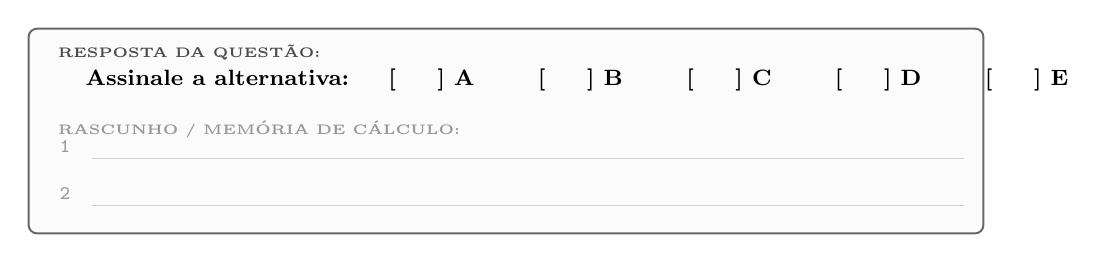
\begin{tikzpicture}
  \draw[rounded corners=3pt, draw=black!60, line width=0.7pt, fill=gray!3] (0,0) rectangle (\linewidth, -2.6cm);
  \node[anchor=north west, font=\tiny\bfseries\color{black!70}] at (0.25cm, -0.08cm) {RESPOSTA DA QUESTÃO:};
  \node[anchor=west, font=\footnotesize\bfseries] at (0.6cm, -0.65cm) {Assinale a alternativa: \quad [ \hspace{0.3cm} ] A \qquad [ \hspace{0.3cm} ] B \qquad [ \hspace{0.3cm} ] C \qquad [ \hspace{0.3cm} ] D \qquad [ \hspace{0.3cm} ] E};
  \node[anchor=north west, font=\tiny\bfseries\color{gray!80}] at (0.25cm, -1.05cm) {RASCUNHO / MEMÓRIA DE CÁLCULO:};
  \draw[gray!35, line width=0.4pt] (0.8cm, -1.65cm) -- (\linewidth-0.25cm, -1.65cm);
  \draw[gray!35, line width=0.4pt] (0.8cm, -2.25cm) -- (\linewidth-0.25cm, -2.25cm);
  \node[anchor=east, font=\scriptsize\ttfamily\color{gray!80}] at (0.65cm, -1.5cm) {1};
  \node[anchor=east, font=\scriptsize\ttfamily\color{gray!80}] at (0.65cm, -2.1cm) {2};
\end{tikzpicture}
\par\vspace{0.2cm}
\fi
